\chapter{Lösungskonzept}
	
	Beim hier verwendeten Entscheidungstemplate handelt es sich um das "<IBM UMF Template for Decision Log"> \cite{hand_ibm_2008}.
	
	\section{Übersicht}
		\eeppi\ soll Entscheidungs-Wissens-Systeme (DKS) mit 
		Projekt-Planungs-Tools (PPT) verbinden.
		
		\begin{figure}[H]
			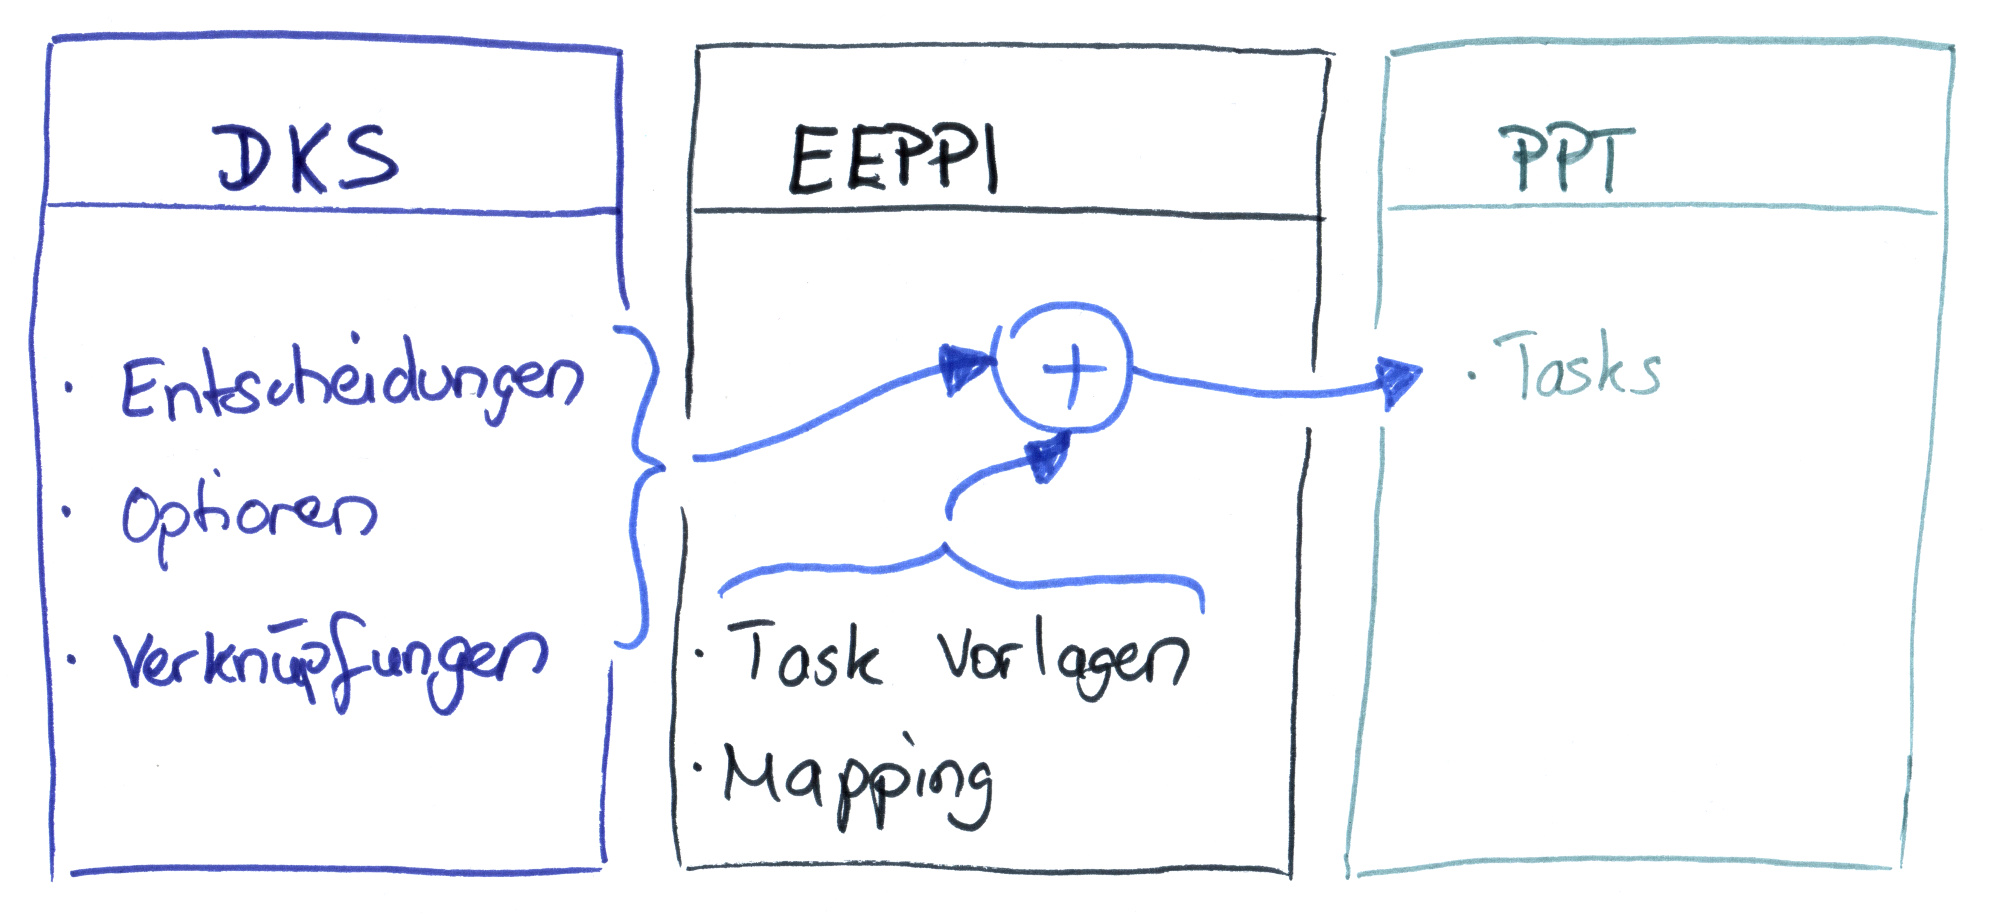
\includegraphics[width=\textwidth]{architecture/media/img/eeppiSchema.jpg}
			\centering
			\caption{Architektur Übersicht}
			\label{fig:architectureSchema}
		\end{figure}	
		
		Dabei sollen Entscheidungen sowie deren verknüpfte Wahlmöglichkeiten (Optionen) mit Taskvorlagen (Tasktemplates) verknüpft werden.
		Diese Verknüpfung wird in folgenden Kapiteln als "<Mapping"> bezeichnet. 
		Anhand diesen Verknüpfungen sollen aus den Aufgabenvorlagen konkrete Aufgaben generiert und in ein \ppt\ übertragen werden.
	
	
	\section{Anbinden der externen Systeme}
		Damit \eeppi\ Daten aus Wissensverwaltungssystemen laden und in \ppt s übertragen kann, muss \eeppi\ an diese angebunden werden können.
		
	
		\subsection{Anbinden von Wissensverwaltungssystemen}
			Beim \cdar\ handelt es sich um ein Wissensverwaltungssystem, 
			das im Rahmen einer Bachelorarbeit an der HSR entwickelt wurde. Mit dem \cdar\ kann ein Benutzer Entscheidungen und und Optionen modellieren und verknüpfen. Das \cdar\ wurde in der Anfangsphase des Projektes als Wissensverwaltungs-Referenzsystem verwendet.
			
		
			Für die Anbindung von \eeppi\ ans \cdar\ gibt es verschiedene Möglichkeiten.
			Wir haben uns für eine eigene Serverkomponente, ein eigenes Userinterface und eine eigene Persistenz entschieden.
			Die Alternativen sowie die Grundlagen dieser Entscheidung sind nachfolgend aufgeführt.
			
			\decision{
				\decisionHeader{INT-CDAR}{Erweiterung \cdar\ / Integration}{Integration}{Architektur design}
			}{
				\decisionContent{Eigene Serverkomponente, eigenes UI (keine UI Integration mit \cdar), eigene Persistenz}
				{In welcher Art soll \eeppi\ mit dem \cdar\ integriert werden?}
				{Die \cdar\ API Stellt alle benötigten Daten zur Verfügung.}
				{Diese Entscheidung beeinflusst die Möglichkeiten der Technologiewahl, der zu nutzenden Schnittstellen und Komponenten und ist daher Grundlegend für weitere Entscheidungen.}
				{
					Jede der Entscheidungen (Serverkomponente, Clientapplikation, Persistenz) kann unabhängig der andern zwei getroffen werden in diesem Fall. Darum sind hier nur die Alternativen der jeweiligen einzelnen Entscheidungen und nicht alle Kombinationen aufgelistet:
					\begin{description}					
						\item[\cdar\ UI erweitern]
						Integration der \eeppi-Funktionalität ins UI des \cdar.			
						\begin{description}
							\item[Vorteile] Nur eine Applikation für Benutzer
							\item[Nachteile] \cdar\ UI muss angepasst werden, \eeppi\ ist vom \cdar\ abhängig
						\end{description}
						
						\item[Serverkomponente ersetzen]
						\eeppi\ bildet eine gemeinsame neue Serverkomponente, die diejenige des \cdar\ ersetzt.
						\begin{description}
							\item[Vorteile] Einheitlichen Unterbau für \cdar\ und \eeppi, nur eine Schnittstelle, nur eine Serverkomponente, einfachere Installation
							\item[Nachteile] Sehr aufwändig, da die \cdar\ Server Komponente viel zu ersetzende Logik beinhaltet, \eeppi\ ist mit \cdar\ gekoppelt.
						\end{description}
						
						\item[\cdar\ Persistenz erweitern]
						\eeppi\ nutzt die Persistenz des \cdar\ und erweitert diese.
						\begin{description}
							\item[Vorteile] Einfachere Wartung, nur eine Persistenz für Backup
							\item[Nachteile] Kopplung von \eeppi\ an \cdar
						\end{description}
					\end{description}
				}
				{
					\eeppi\ soll die \cdar-API zum Laden der Daten benutzen, jedoch eine eigene Server- sowie UI-Komponente und eine eigene Persistenz besitzen. 
					\begin{description}
						\item[Vorteile] \
							\begin{itemize}
								\item Die Persistenz kann im gleichen System wie \cdar\ untergebracht sein, kann aber auch auf einem komplett andern Host laufen.
								\item Es sind keine Anpassungen an \cdar\ notwendig, weder an der Persistenz, der Serverkomponente noch am UI.
								\item \eeppi\ ist Unabhängig vom \cdar\ und könnte auch mit einer andern Applikation als das \cdar\ gekoppelt werden.
							\end{itemize}
						\item[Nachteile] Benutzer müssen zwei Applikationen nutzen (andere URL als \cdar), die Installation ist komplizierter
					\end{description}
				}
				{\cdar\ soll als Referenz-DKS angebunden werden.}
				{Die Schnittstelle für die Datenquelle (Anbindung \cdar) muss generisch und konfigurierbar gestaltet sein.}
				{
					\decisionRef{Tier-Architektur}{ARC-TIERS}, 
					\decisionRef{Server Technologie}{TEC-SERVER}
				}
			}
			
			
			Im Laufe der Prototypenphase wurde seitens der Vertretung der Kundengruppe entschieden, 
			\cdar\ durch eine schlanke Schnittstellenapplikation namens ADRepo zu ersetzen, 
			die ihre Daten über die Enterprise Architect Erweiterung ADMentor bezieht. 
			Diese Veränderung bestätigte die Entscheidung für die gewählte Variante.
			Das Team plante, die Authentisierungsschnittstelle des \cdar\ zu nutzen um Benutzern einen Single Sign On zu ermöglichen.
			Die Ablösung des \cdar\ bedingte allerdings, dass \eeppi\ selbst eine Benutzerverwaltung aufbauen muss.
		
		
		\subsection{Anbinden von \ppt s}
			Entscheidend für die Anbindung eines \ppt\ ist deren Schnittstelle zum Erzeugen von Tasks. 
			Als Referenz-\ppt s haben wir uns für Jira und Redmine entschieden.
			Beide Systeme besitzen solide Schnittstellen,
			die das Verwalten von Tasks erlauben 
			und besitzen einen Verbreitungsgrad über die Softwarebranche hinaus.
		

	\section{Tier-Architektur}
		Die Tier-Architektur wurde zusammen mit der Wahl der Technologie durchgeführt aufgrund der gegenseitigen Einflüsse und Einschränkungen.
		Technologische Entscheidungen werden im Abschnitt \ref{architektur.technologie} auf 
Seite \pageref{architektur.technologie} besprochen.
		
		Aufgrund der Technologischen Möglichkeiten und den anzubindenden Schnittstellen stehen drei mögliche Tier-Architekturen zur Auswahl.
		Die hier verwendeten Begriffe stützen sich auf von Prof. Dr. Zimmermann verwendete Begriffe in der HSR Vorlesung "<Application Architecture"> \cite{prof._dr._zimmerman_layers_2014}.		
		
		\begin{figure}[H]
			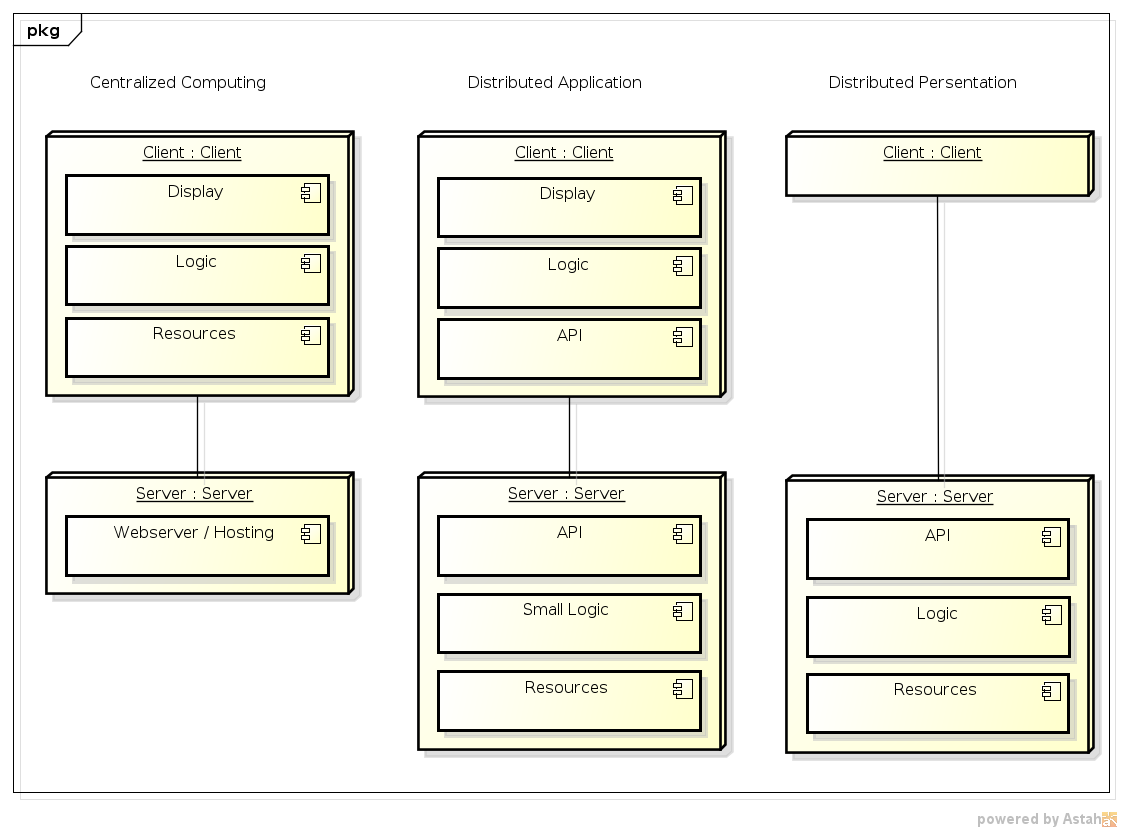
\includegraphics[width=\textwidth]{architecture/media/img/tierArchitecture.png}
			\centering
			\caption{Architektur Varianten}
			\label{fig:tierArchitecture}
		\end{figure}
		\begin{description}
			\item[1-Tier Structure: Centralized Computing (Client-only Application)]
				Die Serverkomponente übernimmt lediglich das Ausliefern einer WebApp. 
				Die WebApp bezieht die Daten direkt aus externen Schnittstellen. 
				Persistenz findet dezentral auf dem Client statt in Form von File Persistence oder 
				Persistence durch das Framework (z.B. HTML5 Storage).
				
			\item[2-Tier Structure: Distributed Application (Single Page App)]
				Die Serverkomponente übernimmt Persistenz sowie minimale Logik (z.B. Login).
				Präsentation und Logik werden von der Client Komponente übernommen.
				
			\item[2-Tier Structure: Distributed Presentation]
				Persistenz, Logik und Präsentation werden vom Server übernommen.
				Die Präsentation wird fertig aufbereitet an den Client gesendet (z.B. HTML Page).
				Es gibt keine aktiven Komponenten auf dem Client, ausgenommen asynchron nachladende Skripte.				
		\end{description}
	
		\decision{
			\decisionHeader{ARC-TIERS}{Tier-Architektur}{Architektur}{Architekturdesign}
		}{
			\decisionContent{Distributed Application (Single Page Application)}
			{Welche Tier-Architektur soll für \eeppi\ gewählt werden?}
			{Die einzusetzende Technologie unterstützt "<Centralized Computing">, "<Distributed Presentation"> und "<Distributed Application">}
			{Diese Entscheidung ist wichtig, damit eine möglichst lose Kopplung \& hohe Flexibilität auch für zukünftige, auf \eeppi\ aufbauende Applikationen, erreicht wird und der Grundstein für Technologieentscheidungen gelegt wird.}
			{"<Centralized Computing">, "<Distributed Presentation">}
			{"<Distributed Application"> ermöglicht eine Serverseitige (zentralisierte) Persistenz sowie den Aufbau einer schnellen und unabhängigen Applikation durch Nutzung der Rechenleistung auf dem Client, sodass der Server und dessen Kosten schlank gehalten werden können.
				Da die App vom Server ausgeliefert wird, kann sie zentral von dort aus verwaltet, gewartet und kontrolliert werden.}
			{keine Speziellen}
			{Die Serverkomponente muss Persistenz sowie eine Datenschnittstelle für den Client bereitstellen.}
			{
				\decisionRef{Server Technologie}{TEC-SERVER}, 
				\decisionRef{Client Framework}{TEC-CLIENT-FW}
			}
		}
		